\documentclass[../main.tex]{subfiles}
\graphicspath{{\subfix{../res/}}}
\begin{document}

We now need to create our pipeline and workflow before we can start building it. The questions we need to answer are : what data are we going to feed into the pipeline and which algorithm are we going to feed?
It is clear that by the results from our state of the art and analysis that not one algorithm must be used in our workflow to achieve the best result. 
To extract as much information and get the possible best results, we have split our system into three inner parts, each with their responsibility, input and output.
But first, let's look into which data we have access to and what to use to feed our system.

\subsection{Feeding data}
\label{subsec:conceptualimplementation_feedingdata}

\begin{figure*}
    \centering
    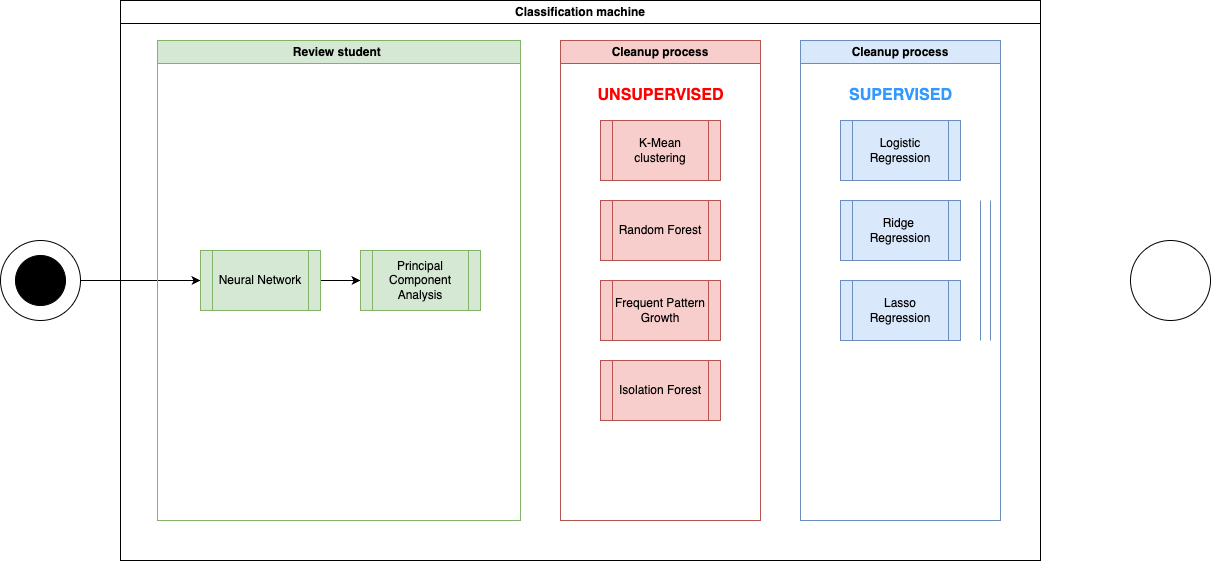
\includegraphics[width=\textwidth]{res//diagram/ML Workflow.png}
    \caption{Machine Learning methodology}
    \label{fig:Machine workflow}
\end{figure*}

\end{document}